\documentclass[a4paper]{article}
\usepackage[left=3cm,right=3cm,top=2cm,bottom=2cm]{geometry} % page settings
\usepackage{enumerate}
\usepackage{hyperref}
\usepackage{graphicx}
\usepackage{amsfonts}
\usepackage{amsthm}
\usepackage{mathtools}
\usepackage{titlesec}
\usepackage{polski}
\usepackage{tikz}
\usepackage[utf8]{inputenc}
\DeclarePairedDelimiter\ceil{\lceil}{\rceil}
\DeclarePairedDelimiter\floor{\lfloor}{\rfloor}
\DeclarePairedDelimiter\set{\lbrace}{\rbrace}


\def\checkmark{\tikz\fill[scale=0.3](0,.35) -- (.25,0) -- (1,.7) -- (.25,.15) -- cycle;} 

\titlespacing*{\subsection}
{0ex}{10ex}{3ex}

\title{Lista 0}
\author{Kamil Matuszewski}
\date{\today}

\begin{document}

\maketitle
\setlength{\parindent}{0.5ex}
\setlength{\parskip}{1.5ex}
\newcommand{\R}{\mathbb{R}}
\newcommand{\N}{\mathbb{N}}


\begin{center}
\begin{tabular}{|c *{6}{|c} |c|}\hline
1 & 2 & 3 & 4 & 5 & 6 & 7 & 8\\
\hline 
0& 0 & \checkmark & \checkmark &\checkmark &\checkmark &\checkmark &\checkmark \\
\hline
\end{tabular}\\
\end{center}

\subsection*{Zadanie 4}
Udowodnić poprawność "mnożenia po rosyjsku".

Zastanówmy się co robi nasz algorytm. Mamy podane liczby $n$ i $m$. W każdym kroku liczbę $n$ dzielimy przez dwa, a liczbę $m$ mnożymy przez dwa. Wykonujemy to dopóki $n \neq 1$. Jeśli w obecnym kroku liczba $n$ jest nieparzysta, dodajemy do całej sumy liczbę $m$ w tym kroku. Ostatecznie suma jest wynikiem mnożenia.\\
Pomyślmy o naszej liczbie $n$ w postaci binarnej. W każdym kroku algorytmu dzielimy ją przez 2 - czyli w rzeczywistości przesuwamy binarnie w lewo, czy inaczej - usuwamy ostatni bit. Jeśli liczba jest nieparzysta - to znaczy, jeśli liczba w zapisie binarnym kończy się na 1 - to do sumy dodajemy liczbę $m$. W i-tym kroku nasza liczba $m$ to tak naprawdę $2^i \cdot m$. Innymi słowy, to, co wykonuje nasz algorytm możemy zapisać jako:
$$\sum\limits_{i=0}^{\log_2{n}}n_i 2^i m$$
Zauważmy, że jeśli i-ty bit liczby $n$ to zero, suma nie jest zwiększona, a jeśli i-ty bit to 1, zwiększamy ją dokładnie o naszą liczbę m w i-tym kroku. Możemy to zapisać inaczej, jako:
$$m \sum\limits_{i=0}^{\log_2{n}}n_i 2^i$$
Teraz, zauważmy, że $\sum\limits_{i=0}^{\log_2{n}}n_i 2^i = n$, i mamy, że nasz algorytm w rzeczywistości liczy $n\cdot m$

Jeśli mówimy o jednorodnym kryterium kosztów, złożoność czasowa naszego algorytmu to $O(\log_2{n})$ - ponieważ w każdym przejściu pętli dzielimy liczbę $n$, mnożymy liczbę $m$ oraz ewentualnie dodajemy do sumy liczbę $m$. Wykonujemy to dokładnie $\log_2{n}$ razy, każde działanie w czasie $O(1)$, stąd taki wynik. Co do złożoności pamięciowej, to jest ona $O(1)$, bo z każdym przejściem programu przechowujemy tylko kolejne liczby.

Jeśli chodzi o logarytmiczne kryterium kosztów, to złożoność czasowa to $\log_2{n}$ czyli pętle, i $\log_2{nm}$ bo w najgorszym wypadku nasza $m$ którą chcemy dodać do sumy ma taką długość, stąd $O(\log_2{n} \log_2{nm})$. Pamięciowo to najdłuższe będą liczby $m$ w $n$'tym kroku i ostateczna suma. Obie mogą mieć maksymalnie $\log_2{nm}$ bitów, stąd, złożoność pamięciowa to $O(\log_2{nm})$

\clearpage
\subsection*{Zadanie 5}
Chcielibyśmy uogólnić algorytm "macierzowy" obliczania n-tej liczby Fibbonacciego na inne ciągi, w których kolejne elementy są liniową kombinacją skończonej liczby elementów wcześniejszych. Inaczej, chcielibyśmy macierz, taką, że:

$$ A\cdot \begin{vmatrix}
a_{k+l-1}\\
\vdots\\
a_k
\end{vmatrix} = \begin{vmatrix}
a_{k+l}\\
\vdots\\
a_{k+1}
\end{vmatrix}$$
Gdzie $a_{k+l}=\alpha_0 a_k + \dots + \alpha_{l} a_{k+l-1}$\\
Można łatwo sprawdzić, że macierz A to:\\

$$\begin{vmatrix}
\alpha_l & \alpha_{l-1} & \dots & \alpha_0\\
1 & 0& \dots & 0\\
0 & 1 & \ddots & 0\\
\vdots &\ddots & \ddots & \vdots\\
0 & 0 & \dots & 1
\end{vmatrix} $$
\clearpage
Teraz, co jeśli n'ty element zależy również od jakiegoś $W(n)$? Sytuacja jest podobna. Teraz:
$$a_n = \alpha_{l} a_{n-1} + \dots + \alpha_{0} a_{n-k} + W(n)$$ gdzie $$W(n)=b_0 n^0 + b_1 n^1 + \dots + b_s n^s$$
Teraz, chcemy macierz A, taką, że:
$$ A\cdot \begin{vmatrix}
a_{n-1}\\
a_{n-2}\\
\vdots\\
a_{n-k}\\
1\\
n^1\\
\vdots\\
n^s
\end{vmatrix} = \begin{vmatrix}
a_{n}\\
a_{n-1}\\
\vdots\\
a_{n-k+1}\\
1\\
(n+1)^1\\
\vdots\\
(n+1)^s
\end{vmatrix}$$

Teraz, można sprawdzić, że:

$$A=\begin{vmatrix}
A_1 & A_2\\
A_3 & A_4
\end{vmatrix} $$
gdzie:
$$A_1=\begin{vmatrix}
\alpha_l & \alpha_{l-1} & \dots & \alpha_0\\
1 & 0& \dots & 0\\
\vdots &\ddots & \ddots & \vdots\\
0 & \dots & 1 & 0\\

\end{vmatrix}$$ 
$$A_2=\begin{vmatrix}
b_0 & b_1 & \dots & b_s\\
0 & 0 & \dots & 0\\
0 & 0 & \ddots & 0\\
\vdots & \ddots & \ddots & \vdots\\
0 & 0 & 0 & 0
\end{vmatrix} \\ $$
$$A_3=0$$
$$A_4=\begin{vmatrix}
{0 \choose 0} & {0 \choose 1} & \dots & {0 \choose s}\\
{1 \choose 0} & {1 \choose 1} & \dots & {1 \choose s}\\
\vdots & \ddots & \ddots & \vdots\\
{s \choose 0} & {s \choose 1} & \dots & {s \choose s}\\
\end{vmatrix}$$ 

Bo, $(n+1)^k = \sum\limits_{i=0}^k {k \choose i} n^i$ więc:
$$\begin{vmatrix}
{0 \choose 0} & 0 & \dots & 0\\
{1 \choose 0} & {1 \choose 1} & \dots & 0\\
\vdots & \ddots & \ddots & \vdots\\
{s \choose 0} & {s \choose 1} & \dots & {s \choose s}\\
\end{vmatrix} \begin{vmatrix}
1\\
n\\
\vdots\\
n^s
\end{vmatrix} = \begin{vmatrix}
1\\
n+1\\
\vdots\\
(n+1)^s
\end{vmatrix}$$

\clearpage

\subsection*{Zadanie 6}
licznik = 0\\
Przejdź po tablicy wykonując:\\
\hspace*{2ex} licznik $\leftarrow$ $a_i \% 2$ XOR licznik\\
Zwróć licznik

Zajmujemy tylko rozmiar tablicy + jeden bit. Jeśli możemy zmieniać na wejściu, zajmujemy tylko długość najdłuższej liczby + jeden bit.

\subsection*{Zadanie 7}
bool=0
Jeśli $u_i=v_i$ to bool = 1, zakończ.\\
Weź z listy parę $(p_i,u_i)$\\
W.P.P.\\
Dopóki $p_i \neq$ korzeń\\
\hspace*{2ex} Jeśli $p_i=v_i$ to bool = 1, zakończ.\\
\hspace*{2ex} W.P.P. weź parę $(x_i,p_i)$; $p_i = x_i$\\
Zakończ.


\textbf{AKTUALIZACJA}

Uwaga, rozwiązanie lepsze:\\
Wcześniej nie zauważyłem, że mamy więcej niż jedno zapytanie. Mamy listę zapytań. Wywoływanie dla każdej pary wierzchołków tego algorytmu jest trochę kosztowne. Dlatego zmienimy rozwiązanie. Przetworzymy nasze drzewo DFS'em i ustalimy dla każdego wierzchołka czas wejścia i czas wyjścia. Oznaczać to będzie, w którym "kroku" weszliśmy do wierzchołka, i w którym musieliśmy się cofnąć do jego rodzica. Stąd na początku czas=0, i z każdym krokiem będzie się zwiększał o 1. Wtedy sprawdzenie czy wierzchołek v leży na ścieżce z u do korzenia, możemy wykonać w czasie O(1), sprawdzając, czy czas wejścia do u jest z przedziału czasu wejścia i wyjścia do v. Przykład: para(x,y) oznacza (czas wejścia, czas wyjścia).\\
\begin{center}
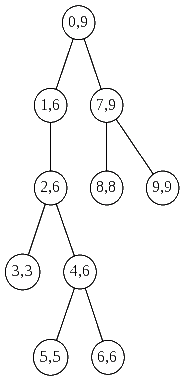
\includegraphics[scale=0.5]{l0przyklad.png}\\
\end{center}
\clearpage
Czas;\\ \\
funkcja Odwiedź(u):\\
\hspace*{2ex}oznacz u jako odwiedzony\\
\hspace*{2ex}czas wejścia u = czas\\
\hspace*{2ex}dla każdego wierzchołka v na liście sąsiedztwa u:\\
\hspace*{4ex}jeżeli v nieodwiedzony:\\
\hspace*{6ex}czas++\\
\hspace*{6ex}Odwiedź(v)\\	
\hspace*{2ex}czas wyjścia u = czas;\\\\
funkcja DFS2(graf G)\\
\hspace*{2ex}Czas=0;\\
\hspace*{2ex}dla każdego wierzchołka u z grafu G:\\
\hspace*{4ex}oznacz u jako nieodwiedzony\\
\hspace*{2ex}Odwiedź(korzeń);\\\\
funkcja CzyLeży(v,u)\\
\hspace*{2ex}Jeśli czas wejścia u $\geq$ czas wejścia v i czas wejścia u $\leq$ czas wyjścia v:\\
\hspace*{4ex}zwróć tak;\\
\hspace*{2ex}zwróć nie;\\

\subsection*{Zadanie 8}
Weźmy ciąg wielomianów $W_0(x), W_1(x), \dots ,W_n(x)$, taki, że\\ $W_0(x)=x$ a $W_k(x)=(W_{k-1}(x)-2)^2$. Czyli mamy: $$W_n(x)=(\dots((x-2)^2-2)^2\dots-2)^2$$
Zauważmy, że chcemy wiedzieć co stoi przy $x^2$. Skoro tak, to w wielomianie $W_k(x)$ nie ma dla nas znaczenia nic poza $a_kx^2 + b_nx + c_n$ (bo tylko z tego w kolejnych wielomianach możemy otrzymać coś przy $x^2$).\\
Weźmy więc $a_kx^2 + b_kx + c_k$. Interesuje nas $a_n$.\\
$a_0=0$ $b_0=1$ $c_0=0$ (bo $W_0(x)=x$).\\
$a_1=1$ $b_1=-4$ $c_1=4$ (bo $W_1(x)=x^2-4x+4$)\\
Sprawdźmy, jak otrzymać kolejne $a_k$:\\
$$(a_kx^2+b_kx+c_k-2)^2=a_k^2x^4 + 2a_kb_kx^3 + (2a_k c_k -4 a_k + b_k^2)x^2 + (2b_kc_k-4b_k)x+(c_k^2-4c_k+4)$$\\
Teraz, mamy:\\
$$c_{k+1}=c_k^2-4c_k+4=(c_k-2)^2$$
Zauważmy, że $c_1=(0-2)^2=4$, $c_3=(4-2)^2=4$, $\dots$ $c_k=4$.\\
Teraz:\\
$$b_{k+1}=2b_kc_k-4b_k=8b_k-4b_k=4b_k$$ $b_1=-4$, $b_2=-4*4$, $\cdots$, $b_k=-4^k$.\\
Teraz:\\
$$a_{k+1}=2a_k c_k -4 a_k + b_k^2=8a_k -4 a_k - 4^k = 4a_k + (-4^k)^2 = 4a_k + 16^k$$
Nadchodzi najciekawsza część: zbudujmy algorytm podobny do algorytmu z zad 5.\\
$$\begin{vmatrix}
4 & 1 \\
0 & 16
\end{vmatrix}\begin{vmatrix}
a_k\\
16^k
\end{vmatrix}=\begin{vmatrix}
a_{k+1}\\
16^{k+1}
\end{vmatrix} $$

Skoro tak, możemy zapisać, że:\\
$$\begin{vmatrix}
4 & 1 \\
0 & 16
\end{vmatrix}^n\begin{vmatrix}
a_0\\
16^0
\end{vmatrix}=\begin{vmatrix}
a_{n}\\
16^{n}
\end{vmatrix} $$
$$\begin{vmatrix}
4 & 1 \\
0 & 16
\end{vmatrix}^n\begin{vmatrix}
0\\
1
\end{vmatrix}=\begin{vmatrix}
a_{n}\\
16^{n}
\end{vmatrix} $$
Jeśli oznaczymy 
$$A=\begin{vmatrix}
a_{11} & a_{12} \\
a_{21} & a_{22}
\end{vmatrix}=\begin{vmatrix}
4 & 1 \\
0 & 16
\end{vmatrix}^n$$
Wtedy, $a_n=a_{12}$ Możemy więc zastosować algorytm szybkiego potęgowania i mamy odpowiedź.

\end{document}
